\documentclass[11pt,a4paper]{article}
\usepackage[margin=2.4cm]{geometry}
\usepackage{graphicx}
\usepackage{amsmath}
\usepackage{xcolor}
\usepackage[colorlinks=true,linkcolor=blue!50!black,urlcolor=blue!50!black]{hyperref}
\graphicspath{{figs/}}

\newcommand{\He}[1]{$^{#1}$He}
\newcommand{\snp}{\sigma_{np}}
\newcommand{\sng}{\sigma_{n\gamma}}

\title{\vspace{-1.2cm}
  {\Large\bfseries The MeV-region capture budget for X17 production at n\_TOF EAR2}\\[2mm]
  {\large What $5\times10^{8}$ fully simulated neutrons (1\,meV--100\,MeV)
   say about moving the analysis window}}
\author{Dylan Neff}
\date{12 June 2026 \\[2mm]
  {\small\itshape Internal note --- informal. Drafted by Claude (Anthropic AI
  assistant) under D.~Neff's direction; \\ simulation, numbers and text
  reviewed by D.~Neff.}}

\begin{document}
\maketitle

\begin{center}
\fcolorbox{black}{yellow!15}{\parbox{0.95\textwidth}{\small
\textbf{Update 2026-07-27 (nose-first + final geometry).} This is the 12 June
draft. \textbf{Production is unchanged} ($\sim$32 X17/day over the MeV region
is gas physics). \textbf{Superseded:} the in-gate detector-background counts
below are pre-final-geometry (STEP LS vessels, 2\,cm plastics, mid-July) --- in
particular the Al-wall term scales $\times0.577$ nose-first ($\sim$255$\to\sim$147
captures/pulse). The recorded-yield / MM-double acceptance / significance
numbers now live in \texttt{angular\_note.tex} (nose-first: acceptance
27.8/27.4\%, Asimov $Z=3.5/6.4\sigma$ July/LS3). See \texttt{CAMPAIGN\_STATUS.md}.}}
\end{center}

%=============================================================================
\section*{Part I --- Summary}

\subsection*{The question}
The thermal note (11 June) showed that the sub-keV X17 measurement is dead:
below 1\,keV the \He{3} gas is opaque to (n,p)t, radiative captures are
capped at $\sng/\snp\approx10^{-8}$ per beam neutron, and the yield is
$\sim$0.1 X17/day --- a factor 50--100 below the rate table. The rescue plan
was always written in the same table: above $\sim$100\,keV the gas is thin,
the thin-target arithmetic is honest there, and those rows carry $\sim$98\%
of the physical rate. \textbf{This note asks whether the full simulation
confirms that promise} --- and delivers the requested curve of expected
X17/day as a function of neutron energy, before detector acceptance.

\subsection*{What we did}
Run B-full fired $5\times10^{8}$ neutrons, sampled from the evaluated EAR2
flux over the \emph{entire} range 1\,meV--100\,MeV with the energy-dependent
transverse beam profile, at the full STEP-derived capsule and detector
geometry (G4NDL high-precision neutron data). Unlike the sub-keV run, here
the radiative channel is measured \emph{directly}: \textbf{714
\He{3}(n,$\gamma$)\He{4} events} were recorded --- 95\% of them above
100\,keV, median $E_n = 1.3$\,MeV. No branching-ratio extrapolation is
needed; the per-decade rate below is simply the direct count.
Normalisation: the sampled flux histogram integrates to
$2.26\times10^{7}$\,n/pulse over the full range (its sub-keV part reproduces
the known $7.31\times10^{6}$ anchor), and $1.929\times10^{4}$ pulses/day.

\subsection*{The answer}
\begin{center}
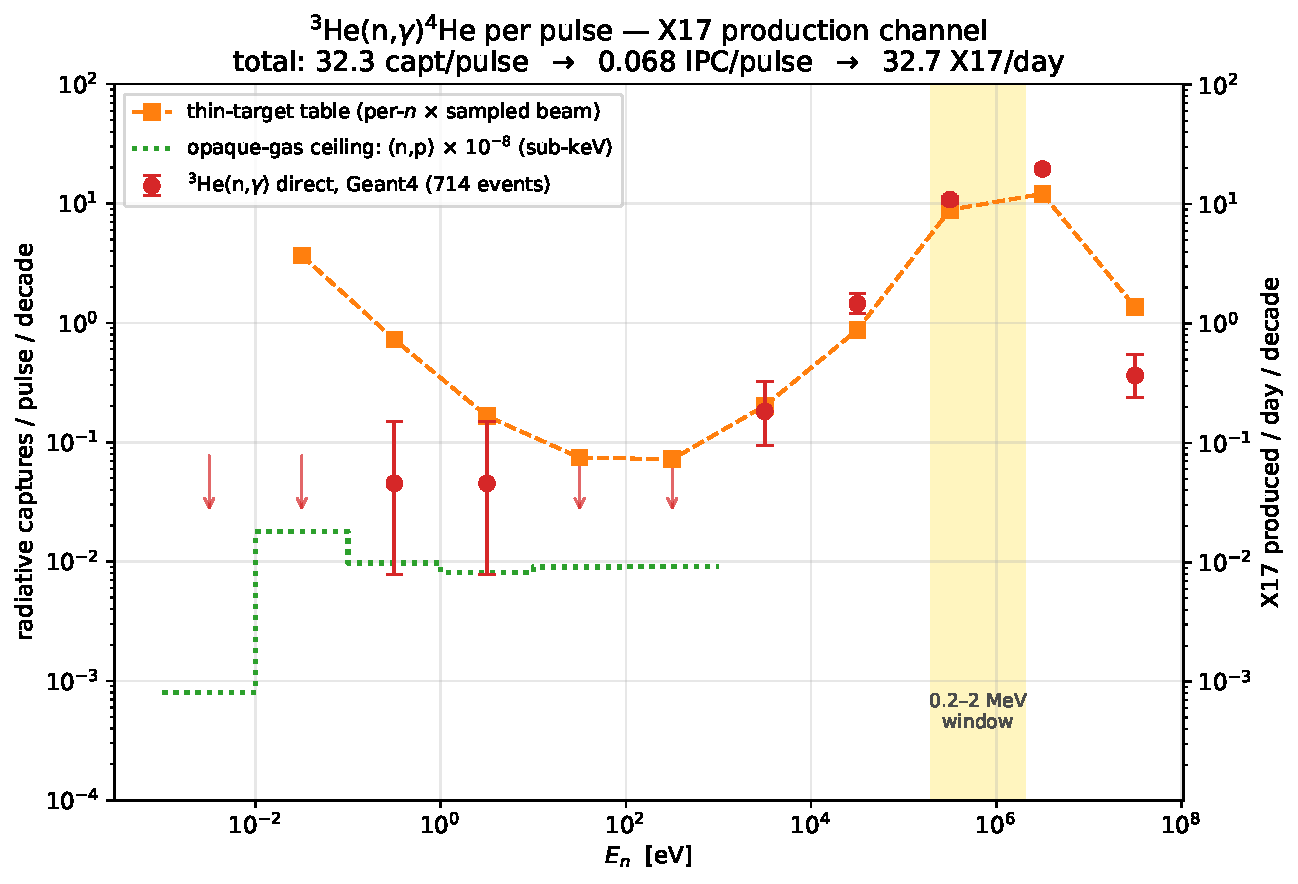
\includegraphics[width=0.94\textwidth]{fig_mev_money.pdf}
\end{center}

\noindent The direct counts (red) tell a complete story in one plot. Below
1\,keV they sit on the opaque-gas ceiling (green), $\times$8--80 under the
table --- the thermal-note result, independently reproduced here (2 events
$\rightarrow$ $0.09$ capt/pulse, vs.\ $(0.5$--$1.1)\times10^{-1}$ from the
dedicated $10^{9}$-event sub-keV run). Above $\sim$10\,keV the data
\emph{meet and slightly exceed} the thin-target table (orange): the gas has
turned thin and the table rows are valid, as claimed. Integrated, with the
2.5\% X17/IPC branching applied \emph{per IPC pair}:

\begin{center}
\begin{tabular}{lcc|cc}
\hline
 & \multicolumn{2}{c|}{per pulse} & \multicolumn{2}{c}{per day} \\
$E_n = 1$\,meV--100\,MeV & 0.2--2\,MeV window & full range
                         & 0.2--2\,MeV window & full range \\
\hline
radiative captures & $22.2\pm1.0$ & $32.3\pm1.2$
                   & $4.3\times10^{5}$ & $6.2\times10^{5}$ \\
IPC pairs ($\times2.1\times10^{-3}$) & $4.7\times10^{-2}$ & $6.8\times10^{-2}$
                   & $899$ & $1309$ \\
X17 (2.5\% of IPC) & $1.2\times10^{-3}$ & $1.7\times10^{-3}$
                   & $\mathbf{22.5\pm1.0}$ & $\mathbf{32.7\pm1.2}$ \\
\hline
\end{tabular}
\end{center}

\noindent\textbf{The bottom line: $\sim$33 X17 produced per day over the
full range, of which $\sim$22.5/day land in the single 0.2--2\,MeV window}
--- before acceptance, trigger and analysis efficiency. That is a factor
$\sim$300 above the sub-keV yield (0.06--0.11/day), and it agrees with the
commented-out 0.2--2\,MeV row of \texttt{results\_3He} (24.9 X17/day) at the
10\% level. Where the table is valid, the full simulation \emph{confirms}
it; per incident neutron Geant4 actually finds $\times$1.2--1.7 \emph{more}
captures than the table's 4-cm-sphere model, consistent with the real
capsule's longer on-axis gas column and scattering re-entry. A 30-day run
produces $\sim$700 X17 decays in the window. \textbf{The measurement moves
from impossible to clearly feasible --- the remaining questions are
acceptance and backgrounds, not production.}

Quoted errors are statistical only. The dominant systematics are inherited
assumptions: the IPC coefficient ($2.1\times10^{-3}$/capture) and the
X17/IPC ratio (2.5\%), both still awaiting provenance from Alberto, and the
flux normalisation (the Ph3 evaluated flux used here is 31\% below the
table's $3.29\times10^{7}$\,n/pulse; per-neutron physics is unaffected).

\subsection*{What's next}
The at-rest pair sample (\texttt{pairs\_v2\_step\_target}, $10^{7}$ events)
gives the detector-response machinery, but MeV captures form \He{4}$^{*}$ at
$E^{*}\approx20.58\,\text{MeV} + \tfrac{3}{4}E_n$ with a CM boost --- the
generator needs $E_n$-dependent kinematics before final acceptance numbers.
In time, the window sits 1.0--3.2\,$\mu$s after the $\gamma$ flash at
EAR2 ($\sim$19.5\,m), sharing the gate with $3\times10^{5}$ (n,p)t and
$9\times10^{4}$ scintillator H-captures per pulse (Sec.~5--6).

%=============================================================================
\clearpage
\section*{Part II --- The full story}

\section{Why the rate comes back at MeV energies}

The sub-keV failure was a competition problem: every neutron is absorbed,
so radiative capture can never beat $\sng/\snp \approx 10^{-8}$. But that
ratio is not a constant of nature --- it is a thermal-energy accident.
$\snp$ falls as $1/v$ while $\sng$ picks up direct-capture strength, so the
branching ratio climbs four orders of magnitude between thermal and MeV:

\begin{center}
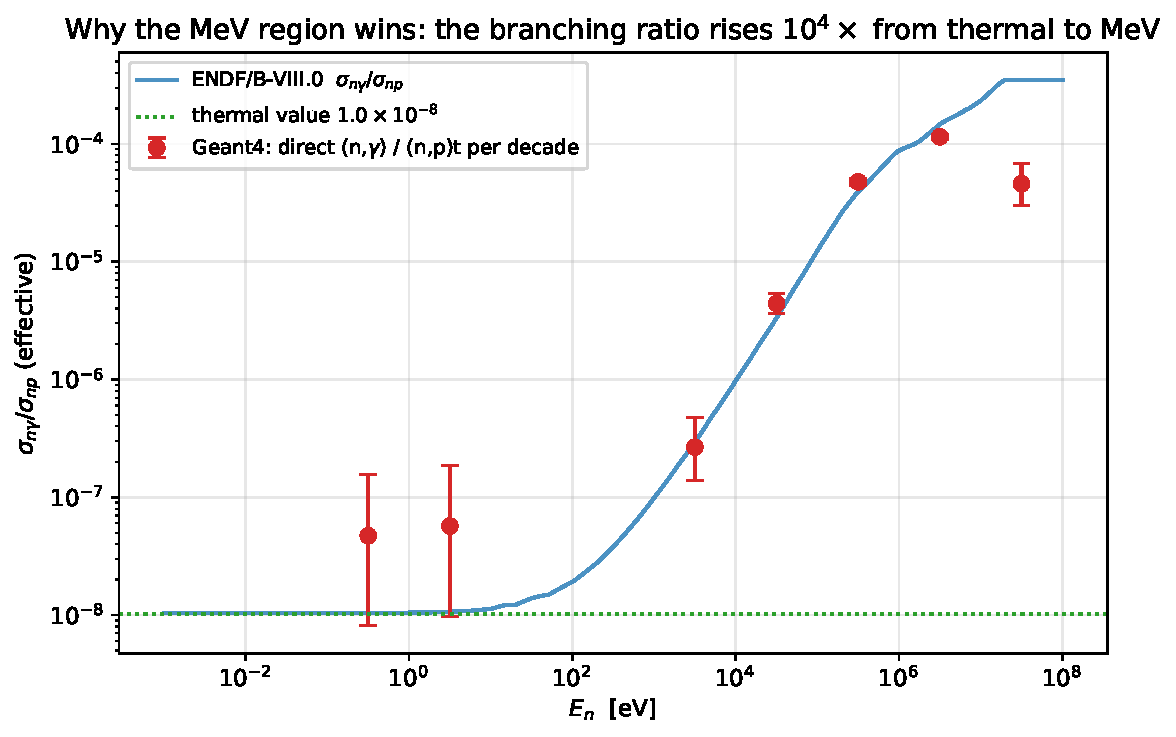
\includegraphics[width=0.8\textwidth]{fig_mev_ratio.pdf}
\end{center}

\noindent The Geant4 per-decade ratios (direct (n,$\gamma$) over (n,p)t,
red) track the ENDF/B-VIII.0 evaluation across six decades --- a
non-trivial closure test of the simulation's neutron physics. (The
10--100\,MeV point falls low: G4NDL data end at 20\,MeV and other channels
open; with 8 events and 0.4 X17/day it is irrelevant to the budget.)
Two things then happen simultaneously above $\sim$100\,keV: the branching
improves by $10^{4}$, \emph{and} the gas stops eating the beam:

\begin{center}
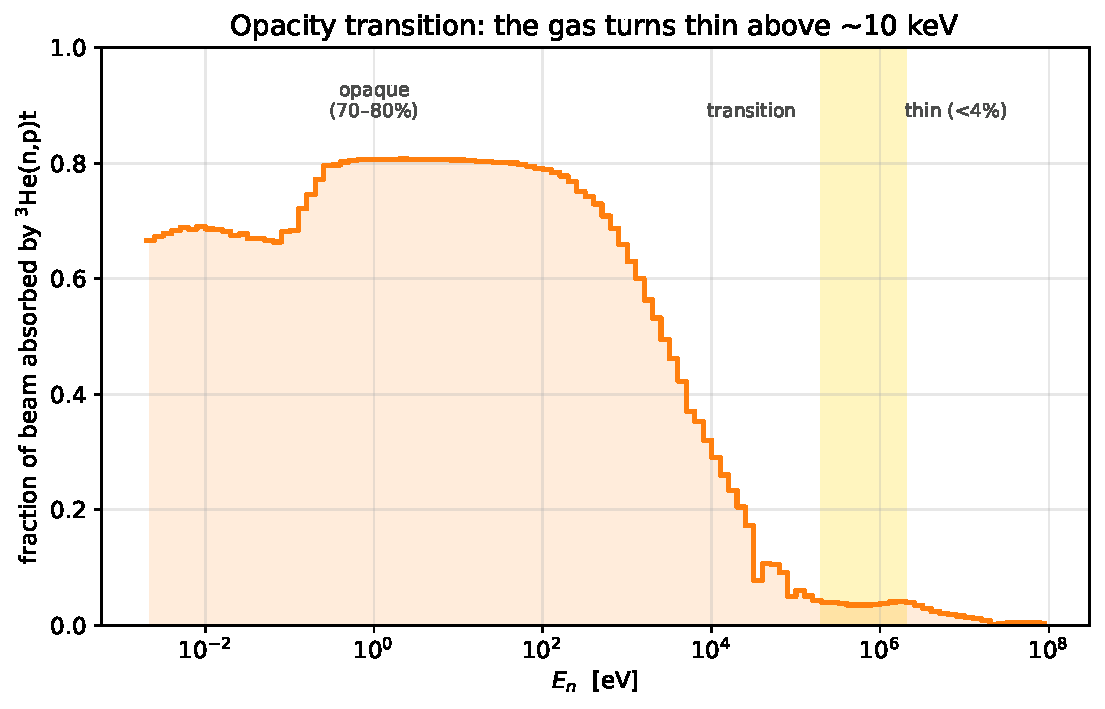
\includegraphics[width=0.8\textwidth]{fig_mev_opacity.pdf}
\end{center}

\noindent Below 1\,keV the gas absorbs 67--81\% of the beam (opaque); by
100\,keV it absorbs $<$4\% (thin). This is the transition the thin-target
table silently assumes --- and above it, the table is right.

\section{The run and its normalisation}

Run B-full: $5\times10^{8}$ events, neutron-beam mode, energies sampled
from \texttt{flux\_n\_pulse\_NOisolet\_100bpd}
(\texttt{data/fluxEAR2-Ph3\_in\_different\_units.root}) over
1\,meV--100\,MeV, transverse positions from the Lambda2D profile, STEP
capsule geometry. All 100 output files validated (tree readable, entry
counts exact). Each simulated neutron carries weight
$w = 2.263\times10^{7}/5\times10^{8} = 4.53\times10^{-2}$ per pulse.

\begin{center}
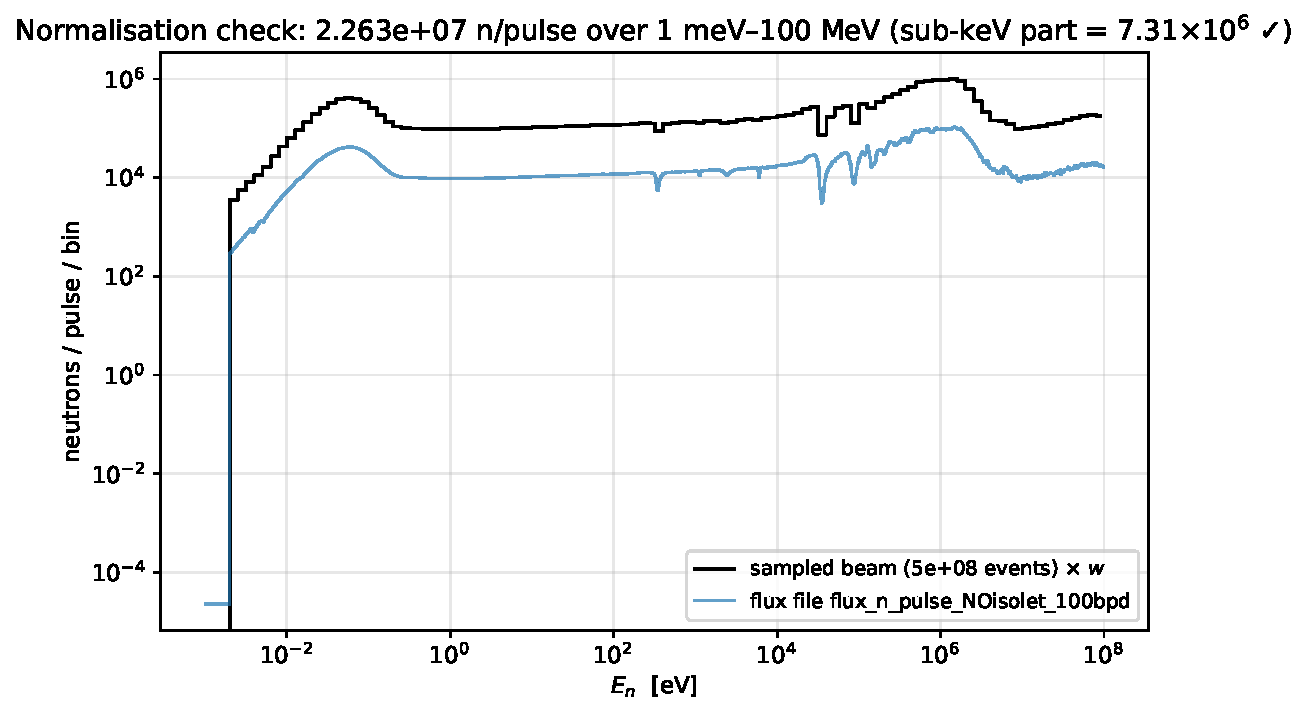
\includegraphics[width=0.8\textwidth]{fig_mev_beam.pdf}
\end{center}

\noindent Two anchor checks: the sampled spectrum reproduces the flux file
bin-by-bin (the generator samples that exact histogram), and the sub-keV
integral is $7.312\times10^{6}$\,n/pulse --- the anchor used throughout the
thermal analysis. Note this evaluated flux is 31\% below the
$3.29\times10^{7}$\,n/pulse assumed in \texttt{results\_3He}; comparisons
with the table are therefore made \emph{per incident neutron}, and per-pulse
rates quoted here are the ones consistent with the Ph3 flux.

\section{The capture budget, decade by decade}

The requested deliverable --- expected X17/day versus neutron energy.
(A pleasant numerical accident: with $\alpha_{\rm IPC}\cdot
{\rm BR}_{\rm X17}\cdot N_{\rm pulses/day} = 2.1\times10^{-3}\times0.025
\times1.929\times10^{4} = 1.01$, captures/pulse and X17/day are numerically
equal, so the table reads either way.)

\begin{center}
\small
\begin{tabular}{lrrrrrr}
\hline
decade & beam/pulse & (n,p)/beam & $N_{n\gamma}$ & capt/pulse & X17/day & G4/table \\
\hline
1\,meV--10\,meV & $1.15\times10^{5}$ & 0.69 & 0 & $<0.08$ & $<0.08$ & --- \\
10\,meV--0.1\,eV & $2.61\times10^{6}$ & 0.67 & 0 & $<0.08$ & $<0.08$ & opaque \\
0.1--1\,eV    & $1.27\times10^{6}$ & 0.76 & 1 & 0.05 & 0.05 & 0.06 \\
1--10\,eV     & $9.85\times10^{5}$ & 0.81 & 1 & 0.05 & 0.05 & 0.27 \\
10--100\,eV   & $1.11\times10^{6}$ & 0.80 & 0 & $<0.08$ & $<0.08$ & opaque \\
0.1--1\,keV   & $1.22\times10^{6}$ & 0.74 & 0 & $<0.08$ & $<0.08$ & opaque \\
1--10\,keV    & $1.45\times10^{6}$ & 0.47 & 4 & 0.18 & 0.18 & 0.90 \\
10--100\,keV  & $2.00\times10^{6}$ & 0.16 & 32 & 1.45 & 1.47 & 1.66 \\
0.1--1\,MeV   & $5.84\times10^{6}$ & 0.039 & 238 & 10.8 & 10.9 & 1.22 \\
1--10\,MeV    & $4.59\times10^{6}$ & 0.037 & 430 & 19.5 & 19.7 & 1.61 \\
10--100\,MeV  & $1.43\times10^{6}$ & 0.006 & 8 & 0.36 & 0.37 & 0.27 \\
\hline
total         & $2.26\times10^{7}$ &  & 714 & 32.3 & 32.7 & \\
\hline
\end{tabular}
\end{center}

\noindent ($N_{n\gamma}$ = direct counts; upper limits are 68\% CL for empty
decades; ``G4/table'' is the ratio of per-neutron capture probabilities.)
Three regimes are visible. \textbf{Opaque} (below $\sim$1\,keV): the
simulation sits far under the table, on the branching-ratio ceiling ---
2 events here vs.\ the table's would-be $\sim$290. \textbf{Transition}
(1--100\,keV): absorption falls from 47\% to 16\%, the table becomes honest
(G4/table $0.9\to1.7$). \textbf{Thin} (above 100\,keV): 95\% of all
production, table confirmed.

\section{Checking the table where it claims validity}

In the two dominant decades the per-neutron agreement is $\times$1.22
(0.1--1\,MeV, 238 events) and $\times$1.61 (1--10\,MeV, 430 events), Geant4
\emph{above} the table. The excess has a mundane reading: the table models a
4\,cm \He{3} sphere ($0.013$\,mm equivalent thickness) in isolation, while
the real capsule presents up to 60\,mm of gas on axis plus a chance for
neutrons scattered in the surrounding apparatus to re-enter. The sign and
size are what one expects, and for planning purposes the conservative number
is the table's own. The 0.2--2\,MeV window integral --- 490 direct events,
$22.2\pm1.0$ capt/pulse --- lands within 10\% of the commented table row
(24.6), the row that originally motivated the move.

\section{The window in time}

\begin{center}
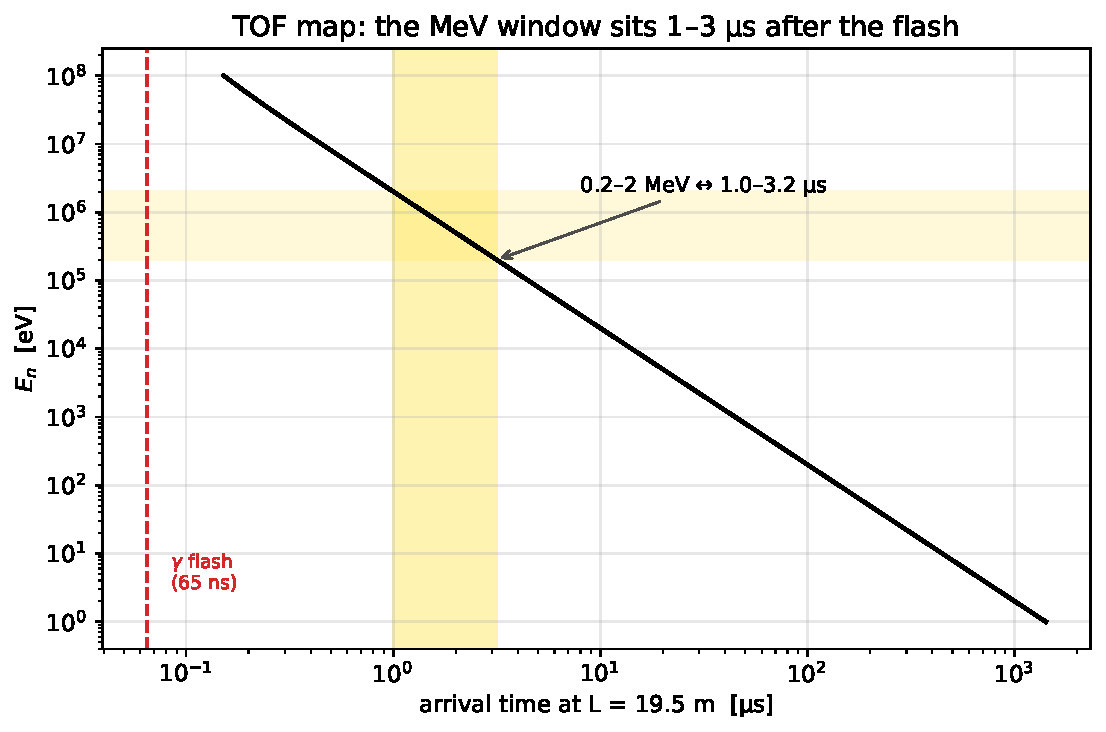
\includegraphics[width=0.78\textwidth]{fig_mev_tof.pdf}
\end{center}

\noindent At EAR2's $\sim$19.5\,m, 0.2--2\,MeV neutrons arrive
1.0--3.2\,$\mu$s after production --- a 2.2\,$\mu$s gate, 15--50 flash
transit times after the $\gamma$ flash (65\,ns). Whether the detectors have
recovered from the flash by 1\,$\mu$s is an \emph{experimental} question
this simulation cannot answer (the flash itself is not modelled); it is the
single most important measurement to make with the real setup. Within the
gate, per pulse, the simulation puts: $3.0\times10^{5}$ (n,p)t events in the
gas (764\,keV of charged heat each --- the dominant in-window energy
deposition), $8.8\times10^{4}$ H-captures in the liquid scintillator
(2.2\,MeV $\gamma$, born \emph{inside} the calorimeter), $2.6\times10^{3}$
plastic-veto captures and $\sim$255 Al-wall captures (7.7\,MeV cascades;
nose-first $\sim$147, $\times0.577$).
The signal: 22 IPC-capable captures per pulse, of which
$4.7\times10^{-2}$ produce a pair. Pile-up and trigger design at
$\mu$s timescales, not raw rate, will set the sensitivity.

\section{Backgrounds across the spectrum}

\begin{center}
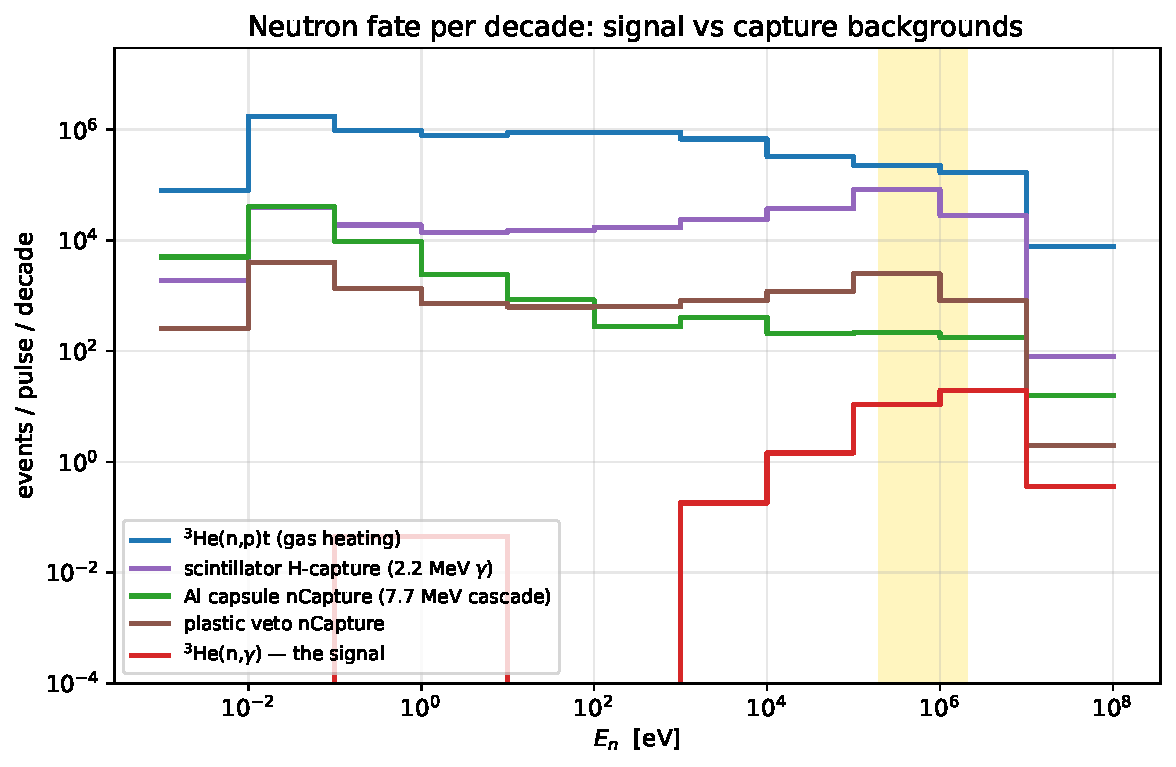
\includegraphics[width=0.85\textwidth]{fig_mev_backgrounds.pdf}
\end{center}

\noindent The full-range hierarchy per pulse: 67\% of the beam escapes
without a terminal interaction (mostly fast neutrons punching through the
thin gas), 30\% undergoes (n,p)t (concentrated sub-keV, where the
late-arriving neutrons deposit their heat tens of $\mu$s to ms after the
window of interest --- a slow-tail rate issue, not an in-window one), and
the leading capture backgrounds are the liquid-scintillator H-captures
($2.8\times10^{5}$/pulse) and Al-capsule captures ($6.0\times10^{4}$/pulse)
--- the same two channels flagged in the thermal note, now quantified over
the full spectrum. Run C (biased wall-$\gamma$ source) remains the right
tool to turn these counts into calorimeter spectra.

\section{What is still assumed}

\begin{enumerate}
  \item \textbf{IPC coefficient} $2.1\times10^{-3}$/capture and
    \textbf{X17/IPC = 2.5\%}: flat values from \texttt{results\_3He},
    provenance (multipolarity, $E^{*}$ dependence) still to be confirmed
    with Alberto. Every per-day X17 number scales linearly with both.
  \item \textbf{Kinematics}: MeV captures form \He{4}$^{*}$ at
    $E^{*} = 20.58\,\text{MeV} + \tfrac{3}{4}E_n$ (+ CM boost): at 2\,MeV
    that is 1.5\,MeV of extra excitation and a boosted decay frame ---
    opening angle, energy sharing and TOF of the pair all shift. The
    existing at-rest pair sample is the right machinery test but the wrong
    final answer; the generator extension is the gating item for run A.
  \item \textbf{Acceptance}: nothing here includes the detector. The next
    step is \texttt{analyze\_pairs.py} on \texttt{pairs\_v2\_step\_target}
    ($10^{7}$ events, current STEP geometry) for the baseline response
    matrix.
  \item \textbf{Above 20\,MeV}: G4NDL ends; that decade is model-dependent
    and contributes 1\% of the budget.
  \item \textbf{Gamma-flash recovery}: not simulated; must come from beam
    data.
\end{enumerate}

\section{Where this leaves us}

The energy budget argument is settled: \textbf{the X17 production rate at
EAR2 is $\sim$33/day, it lives at MeV energies, and the single 0.2--2\,MeV
window carries $\sim$22/day} --- $\times$300 the sub-keV yield, in
10\%-level agreement with the rate table where the table is valid. The
program is now an acceptance-and-backgrounds problem:

\begin{enumerate}
  \item Pairs acceptance on the at-rest sample (machinery + baseline).
  \item Generator extension to $E_n$-dependent kinematics; re-plan run A.
  \item Gamma-flash recovery measurement at EAR2; trigger/pile-up design
    for a 1--3\,$\mu$s gate ($3\times10^{5}$ (n,p) + $10^{5}$ capture
    $\gamma$s per pulse in-gate).
  \item Run C (wall-$\gamma$ spectra) and run D (single-particle response)
    as planned.
  \item Alberto: confirm $\alpha_{\rm IPC}$, X17/IPC, and reconcile the
    31\% flux-normalisation difference.
\end{enumerate}

%=============================================================================
\appendix
\section*{Appendix: reproduction}

\begin{itemize}
  \item Scan (lxplus, $\sim$20\,min, 8 workers):
    \texttt{python3 scripts/analyze\_mev\_captures.py
    /eos/experiment/ntof/data/x17/full\_sim/neutrons\_fullrange/ -o
    mev\_captures --workers 8}
  \item Rates + figures (local or lxplus):
    \texttt{python3 scripts/make\_mev\_report\_figures.py} reads
    \texttt{analysis/mev/mev\_captures.npz}, writes
    \texttt{analysis/mev/mev\_rates.json} and \texttt{docs/report/figs/}.
  \item Raw scan output: \texttt{analysis/mev/mev\_captures.npz}
    (110-bin histograms, terminal-interaction budget, 714 individual
    (n,$\gamma$) energies). Derived rates: \texttt{analysis/mev/mev\_rates.json}.
  \item Pitfalls inherited from the thermal campaign: \He{3}(n,p)t appears
    as \texttt{neutronInelastic} (not \texttt{nCapture}); the 2.5\% X17
    branching is per IPC pair, not per capture; \emph{the thermal
    $\sng/\snp = 10^{-8}$ must never be applied outside the sub-keV region}
    (it is wrong by $10^{3}$--$10^{4}$ at MeV --- use the direct counts).
\end{itemize}

\end{document}
